\documentclass{article}
\usepackage[margin=1in]{geometry}
\usepackage{amsmath}
\usepackage{amssymb}
\usepackage{amsthm}
\usepackage{bm}
\usepackage{hyperref}
\usepackage{graphicx}
\usepackage{caption}
\usepackage{listings}
\usepackage{xcolor}
\usepackage{float}
\usepackage{placeins}
\graphicspath{{figures/}}

% Code style
\lstdefinestyle{code}{
  basicstyle=\ttfamily\small,
  numbers=left,
  numberstyle=\tiny,
  numbersep=8pt,
  keywordstyle=\color{blue},
  commentstyle=\color{teal!70!black},
  stringstyle=\color{orange!70!black},
  showstringspaces=false,
  breaklines=true,
  frame=single,
  framerule=0.3pt,
  rulecolor=\color{black!15}
}
\lstset{style=code}

\title{Generative Models: Autoencoders, Adversarial Networks, and Diffusion}
\author{}
\date{\today}

\begin{document}
\maketitle
\tableofcontents
\FloatBarrier

\section{Autoencoders (AE, VAE)}
Autoencoders learn latent representations by reconstructing inputs. The encoder $f_\phi$ maps $\mathbf{x}$ to latent code $\mathbf{z}$, and the decoder $g_\theta$ reconstructs $\hat{\mathbf{x}}$. Figure~\ref{fig:autoencoder_architecture} illustrates the bottleneck structure.

\subsection{Deterministic Autoencoders}
The reconstruction loss (often mean squared error) is
\begin{equation}
  \mathcal{L}_{\mathrm{AE}}(\theta, \phi) = \frac{1}{N} \sum_{i=1}^{N} \left\| g_\theta \bigl(f_\phi(\mathbf{x}_i)\bigr) - \mathbf{x}_i \right\|_2^2.
\end{equation}
While AEs excel at dimensionality reduction, latent spaces may be discontinuous. Regularized variants enforce structure:
\begin{itemize}
  \item \textbf{Sparse AE:} Adds $L_1$ penalties on activations to encourage sparse latent representations.
  \item \textbf{Denoising AE:} Trains with corrupted inputs $\tilde{\mathbf{x}}$ but reconstructs the clean $\mathbf{x}$, enhancing robustness.
  \item \textbf{Contractive AE:} Penalizes the Jacobian $\| \nabla_{\mathbf{x}} f_\phi(\mathbf{x}) \|_F^2$ to learn invariant features.
\end{itemize}

\subsection{Variational Autoencoders}
VAEs impose a probabilistic latent variable model. Given prior $p(\mathbf{z}) = \mathcal{N}(\mathbf{0}, \mathbf{I})$ and decoder likelihood $p_\theta(\mathbf{x} \mid \mathbf{z})$, the evidence lower bound (ELBO) for each sample is
\begin{equation}
  \log p_\theta(\mathbf{x}) \ge \mathbb{E}_{q_\phi(\mathbf{z} \mid \mathbf{x})} \bigl[\log p_\theta(\mathbf{x} \mid \mathbf{z})\bigr] - \mathrm{KL}\bigl(q_\phi(\mathbf{z} \mid \mathbf{x}) \,\|\, p(\mathbf{z})\bigr).
\end{equation}
Parameterizing $q_\phi(\mathbf{z} \mid \mathbf{x}) = \mathcal{N}\bigl(\boldsymbol{\mu}_\phi(\mathbf{x}), \operatorname{diag}(\boldsymbol{\sigma}^2_\phi(\mathbf{x}))\bigr)$ enables reparameterization:
\begin{equation}
  \mathbf{z} = \boldsymbol{\mu}_\phi(\mathbf{x}) + \boldsymbol{\sigma}_\phi(\mathbf{x}) \odot \boldsymbol{\epsilon}, \quad \boldsymbol{\epsilon} \sim \mathcal{N}(\mathbf{0}, \mathbf{I}).
\end{equation}
The KL term has closed form:
\begin{equation}
  \mathrm{KL} = -\tfrac{1}{2} \sum_{j=1}^{d} \left(1 + \log \sigma_j^2 - \mu_j^2 - \sigma_j^2 \right).
\end{equation}

\subsection{Beta-VAE and Disentanglement}
$\beta$-VAE scales the KL divergence, $\mathcal{L} = \mathbb{E}[\log p_\theta(\mathbf{x} \mid \mathbf{z})] - \beta\, \mathrm{KL}(q_\phi \| p)$, promoting disentangled latent factors when $\beta > 1$. Mutual information penalties and Total Correlation regularizers (TC-VAE) refine latent independence.

\subsection{Training Procedure}
\begin{lstlisting}[language=Python, caption={Variational autoencoder training loop with KL annealing.}]
for epoch in range(num_epochs):
    beta = min(1.0, epoch / kl_warmup_epochs)
    for x in dataloader:
        mu, logvar = encoder(x)
        z = mu + torch.exp(0.5 * logvar) * torch.randn_like(mu)
        x_recon = decoder(z)
        recon_loss = reconstruction_criterion(x_recon, x)
        kl = -0.5 * (1 + logvar - mu.pow(2) - logvar.exp()).sum(dim=1).mean()
        loss = recon_loss + beta * kl
        loss.backward()
        optimizer.step()
        optimizer.zero_grad()
\end{lstlisting}

\begin{figure}[H]
  \centering
  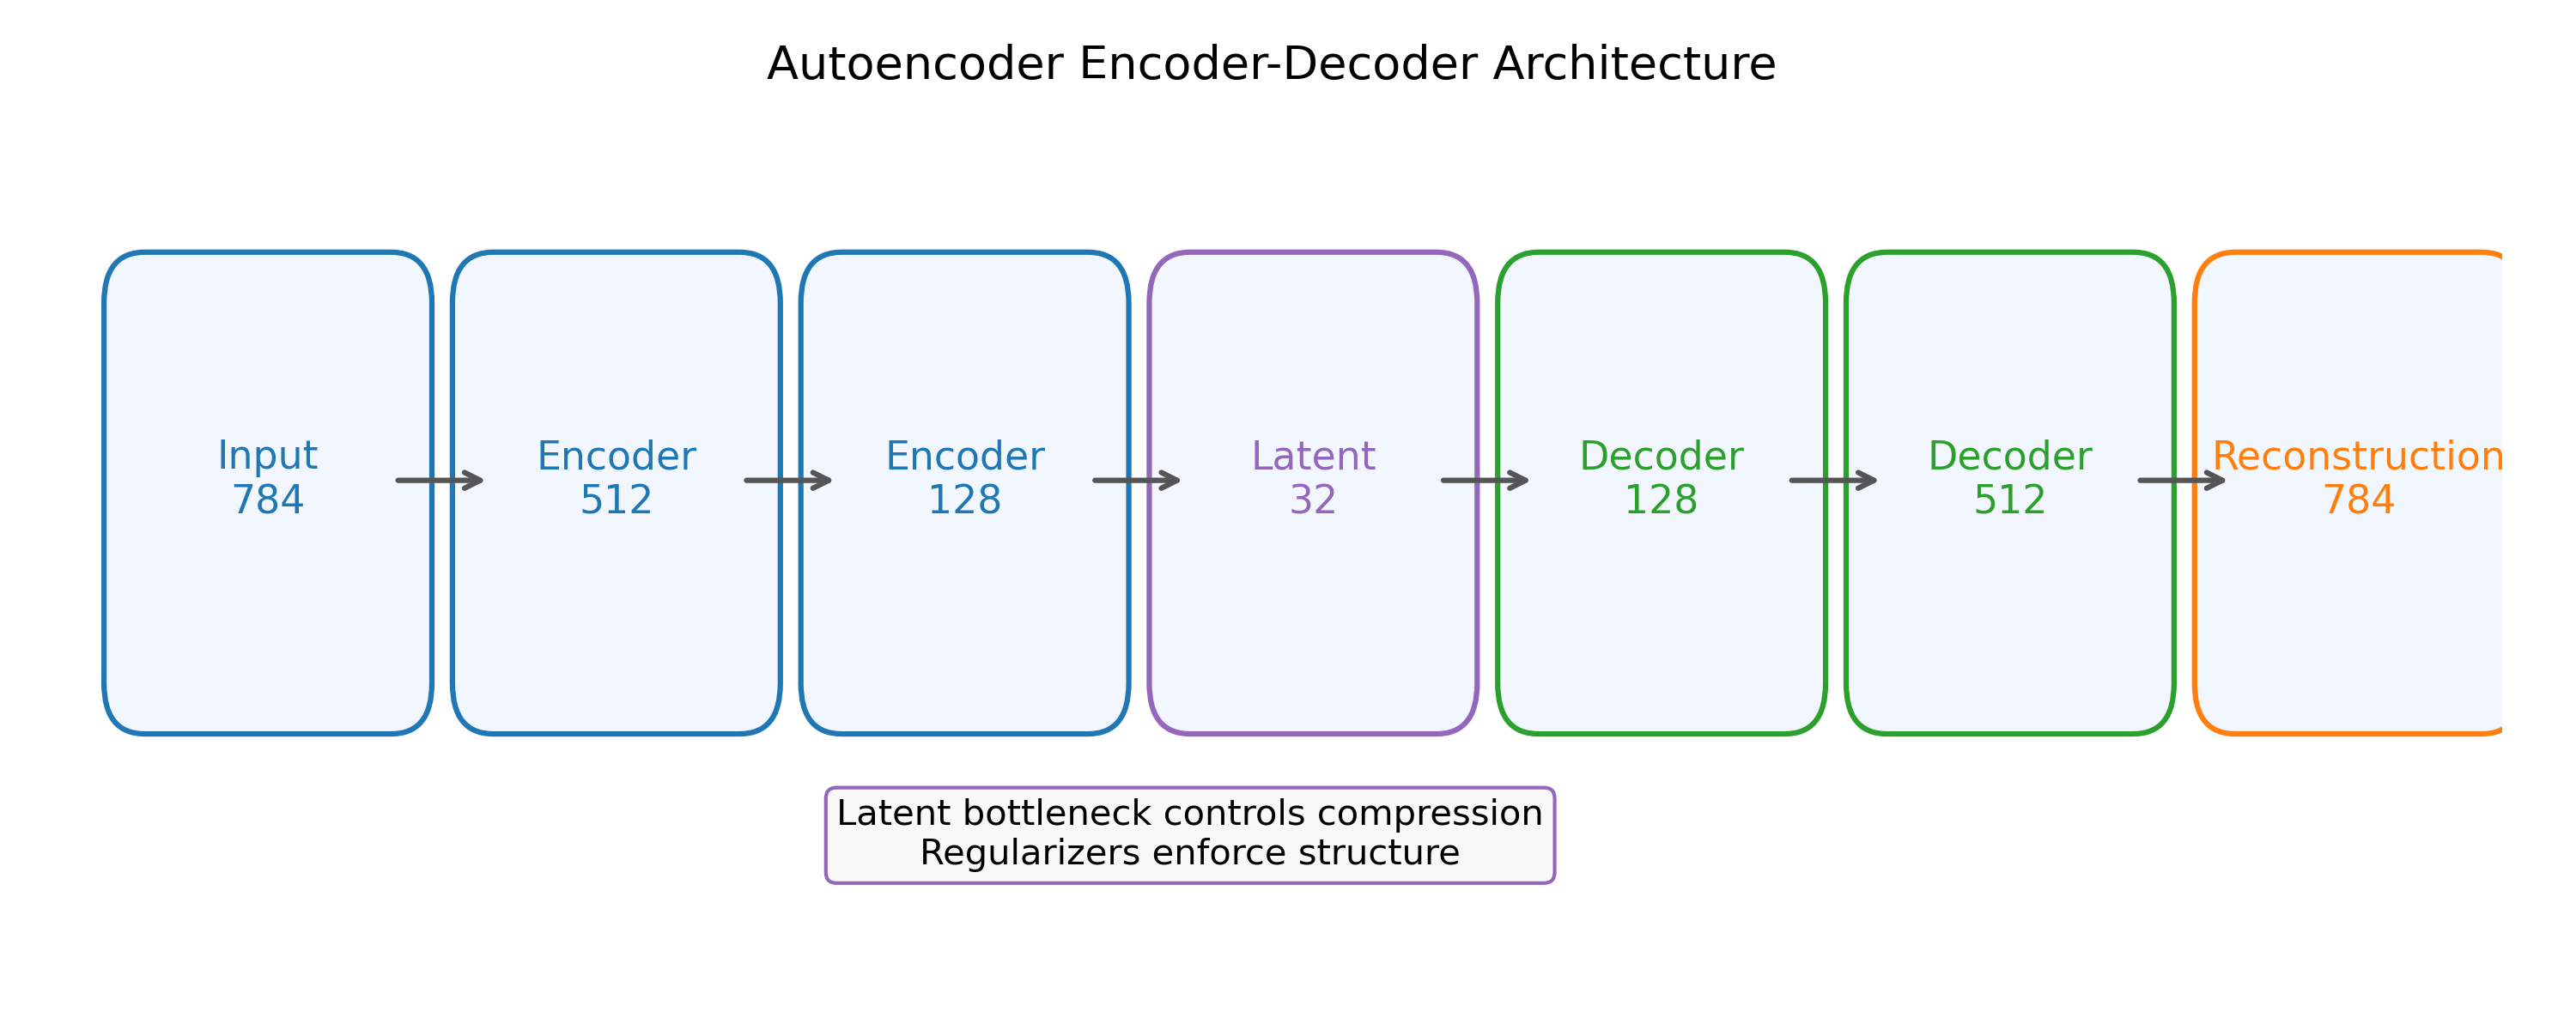
\includegraphics[width=0.8\textwidth]{autoencoder_architecture.png}
  \caption{Autoencoder architecture with deterministic encoder/decoder. Bottleneck dimensionality controls compression.}
  \label{fig:autoencoder_architecture}
\end{figure}

\begin{figure}[H]
  \centering
  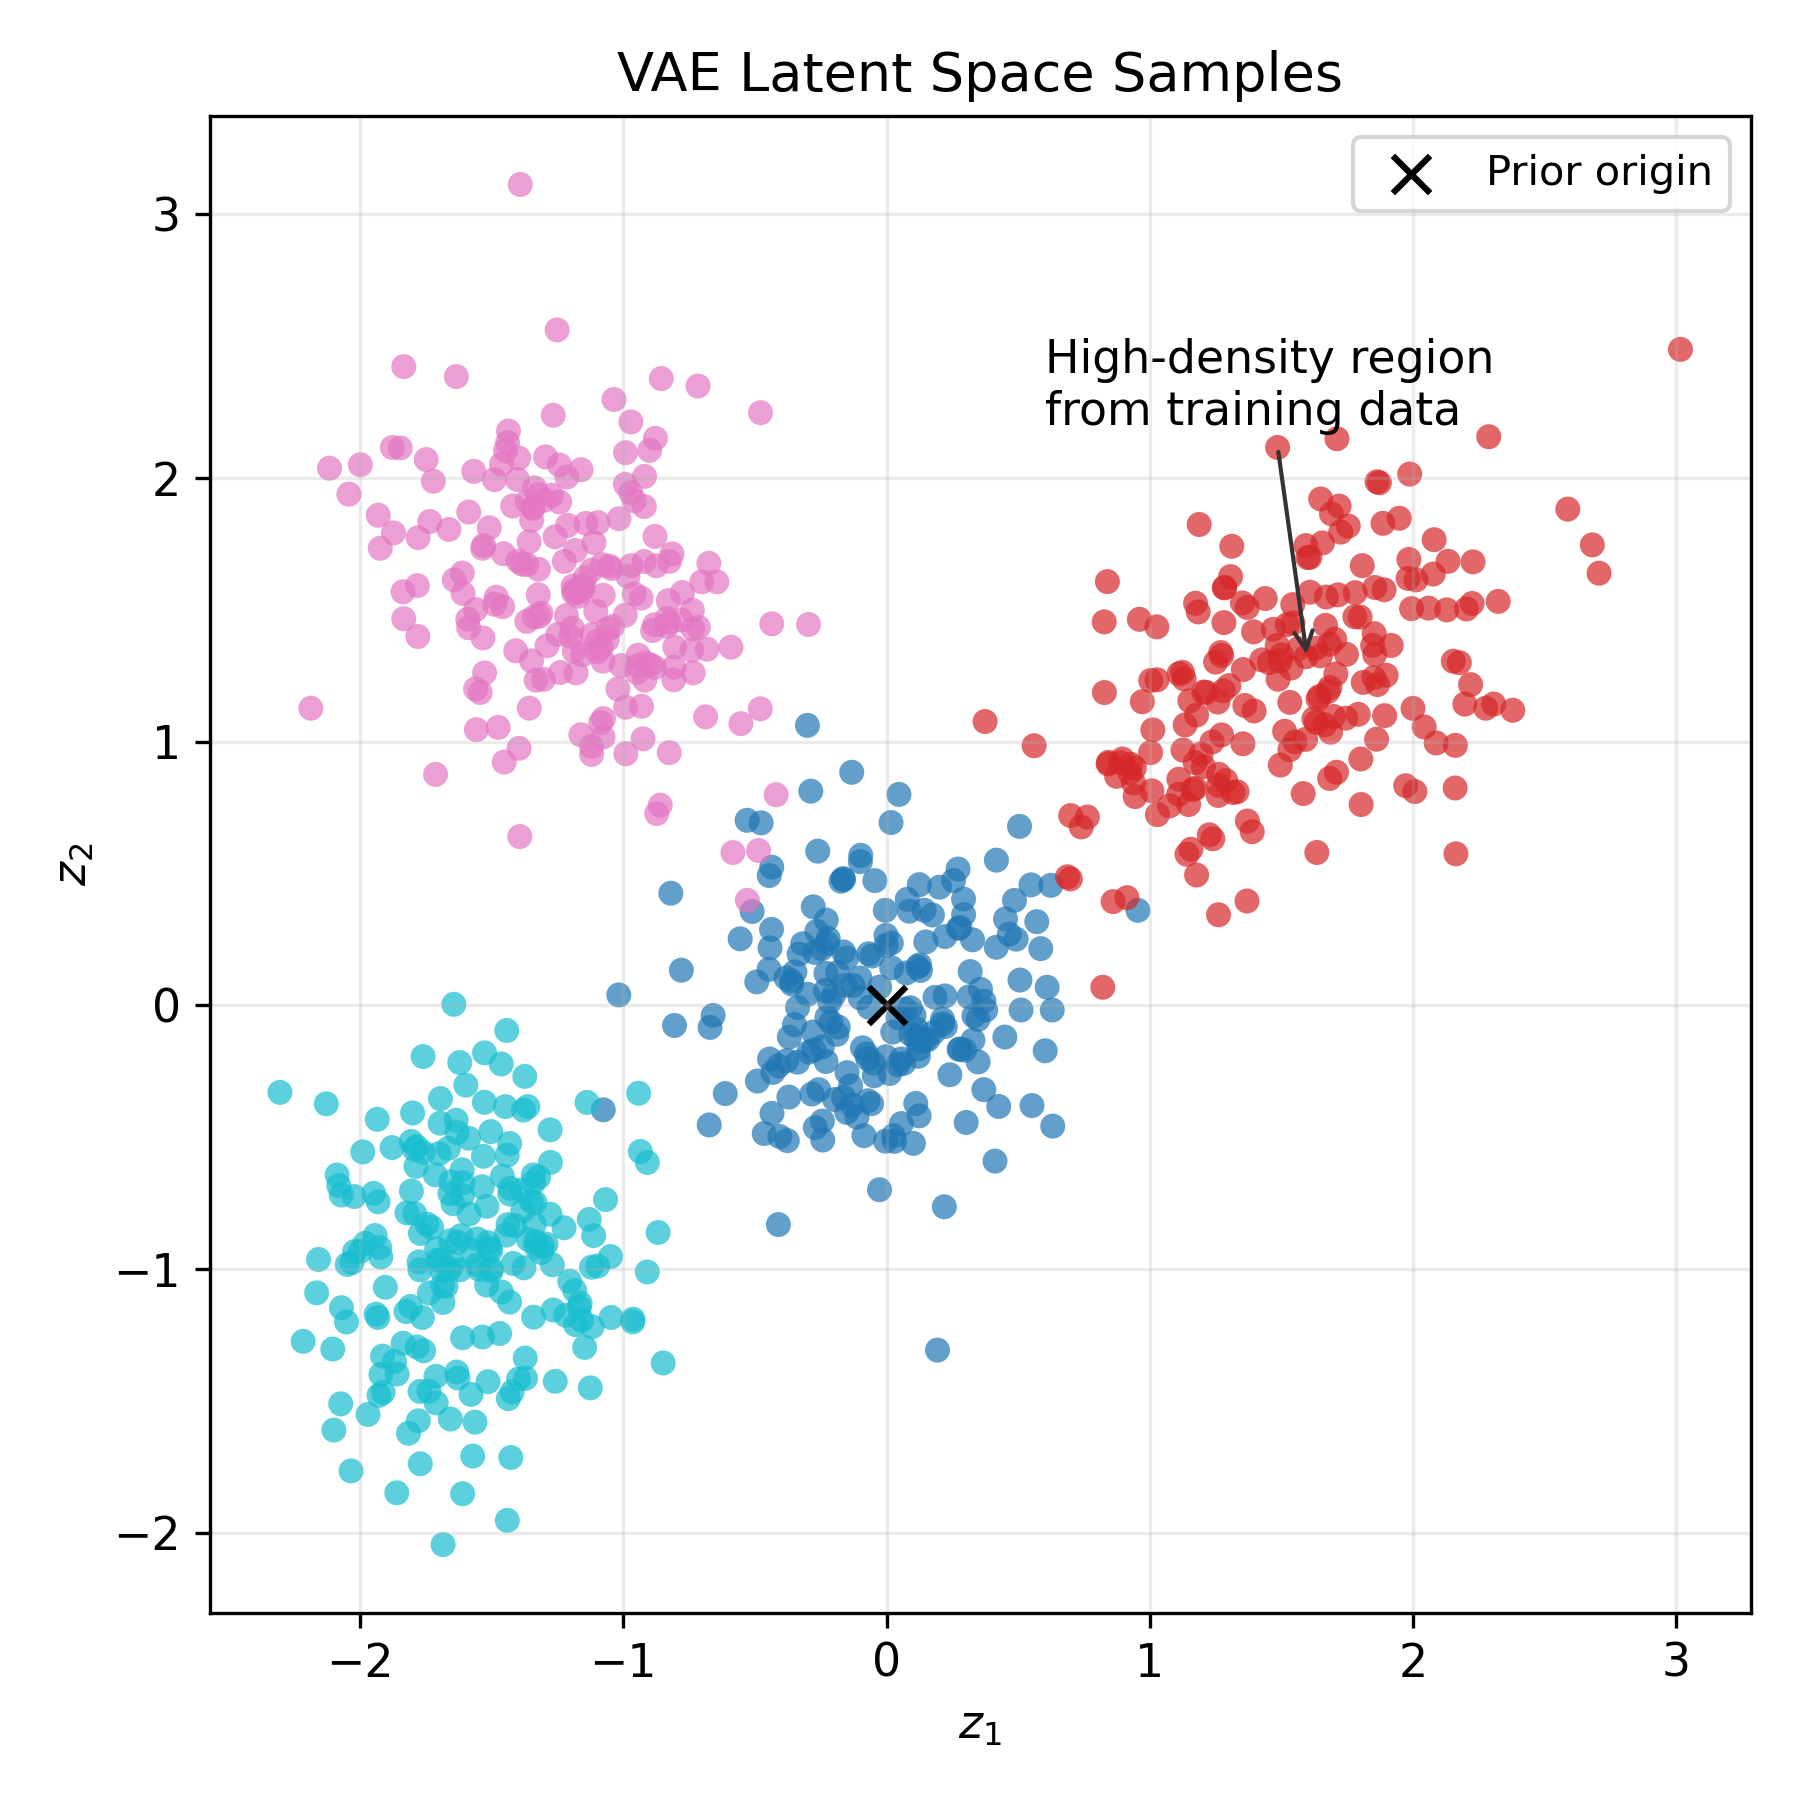
\includegraphics[width=0.8\textwidth]{vae_latent_space.png}
  \caption{Latent space sampling in a VAE. Points near the origin correspond to plausible reconstructions.}
  \label{fig:vae_latent_space}
\end{figure}
\FloatBarrier

\section{Generative Adversarial Networks (GANs)}
GANs pit a generator $G$ against a discriminator $D$. The min-max objective,
\begin{equation}
  \min_{G} \max_{D} \; \mathbb{E}_{\mathbf{x} \sim p_{\mathrm{data}}} \bigl[\log D(\mathbf{x})\bigr] + \mathbb{E}_{\mathbf{z} \sim p(\mathbf{z})} \bigl[\log (1 - D(G(\mathbf{z})))\bigr],
\end{equation}
drives $G$ to synthesize realistic samples. Figure~\ref{fig:gan_training_dynamics} depicts loss curves and mode coverage.

\subsection{GAN Variants}
\begin{itemize}
  \item \textbf{DCGAN:} Convolutional architectures with strided convolutions, batch normalization, and ReLU/Leaky ReLU activations for stable image synthesis.
  \item \textbf{WGAN and WGAN-GP:} Replace Jensen-Shannon divergence with Earth-Mover distance. The WGAN objective
  \begin{equation}
    \min_{G} \max_{D \in \mathcal{D}_1} \; \mathbb{E}_{\mathbf{x} \sim p_{\mathrm{data}}} [D(\mathbf{x})] - \mathbb{E}_{\mathbf{z} \sim p(\mathbf{z})} [D(G(\mathbf{z}))],
  \end{equation}
  constrains $D$ to 1-Lipschitz. Gradient penalty adds $\lambda (\|\nabla_{\hat{\mathbf{x}}} D(\hat{\mathbf{x}})\|_2 - 1)^2$ to encourage Lipschitz continuity.
  \item \textbf{StyleGAN:} Introduces style-based modulation. Latent $\mathbf{w}$ modulates convolution kernels via adaptive instance normalization, enabling control over coarse-to-fine features. Path-length regularization and noise injection improve fidelity.
\end{itemize}

\subsection{Training Stabilization}
Mode collapse, vanishing gradients, and discriminator overpowering require safeguards:
\begin{itemize}
  \item Feature matching and minibatch discrimination regularize $G$.
  \item Spectral normalization enforces Lipschitz constraints by rescaling weight matrices.
  \item Two-time-scale update rule (TTUR) adjusts learning rates $(\eta_D, \eta_G)$ to balance convergence.
\end{itemize}

\subsection{Evaluation Metrics}
Fréchet Inception Distance (FID) approximates the Wasserstein-2 distance between Inception features:
\begin{equation}
  \mathrm{FID} = \|\boldsymbol{\mu}_r - \boldsymbol{\mu}_g\|_2^2 + \mathrm{Tr}\left(\boldsymbol{\Sigma}_r + \boldsymbol{\Sigma}_g - 2(\boldsymbol{\Sigma}_r \boldsymbol{\Sigma}_g)^{1/2}\right).
\end{equation}
Precision/recall for generative models and Inception Score complement FID.

\subsection{StyleGAN2 Generator Forward Pass}
\begin{lstlisting}[language=Python, caption={Simplified StyleGAN2 generator block with style modulation.}]
class StyledConv(nn.Module):
    def __init__(self, in_channels, out_channels, style_dim, upsample):
        super().__init__()
        self.upsample = upsample
        self.weight = nn.Parameter(torch.randn(1, out_channels, in_channels, 3, 3))
        self.modulation = nn.Linear(style_dim, in_channels)
        self.noise_weight = nn.Parameter(torch.zeros(1, out_channels, 1, 1))
        self.activation = nn.LeakyReLU(0.2)

    def forward(self, x, style, noise):
        style = self.modulation(style).view(-1, 1, x.size(1), 1, 1)
        weight = self.weight * (style + 1e-8)
        if self.upsample:
            x = upsample_2x(x)
        x = conv2d_modulated(x, weight)
        x = x + self.noise_weight * noise
        return self.activation(x)
\end{lstlisting}

\begin{figure}[H]
  \centering
  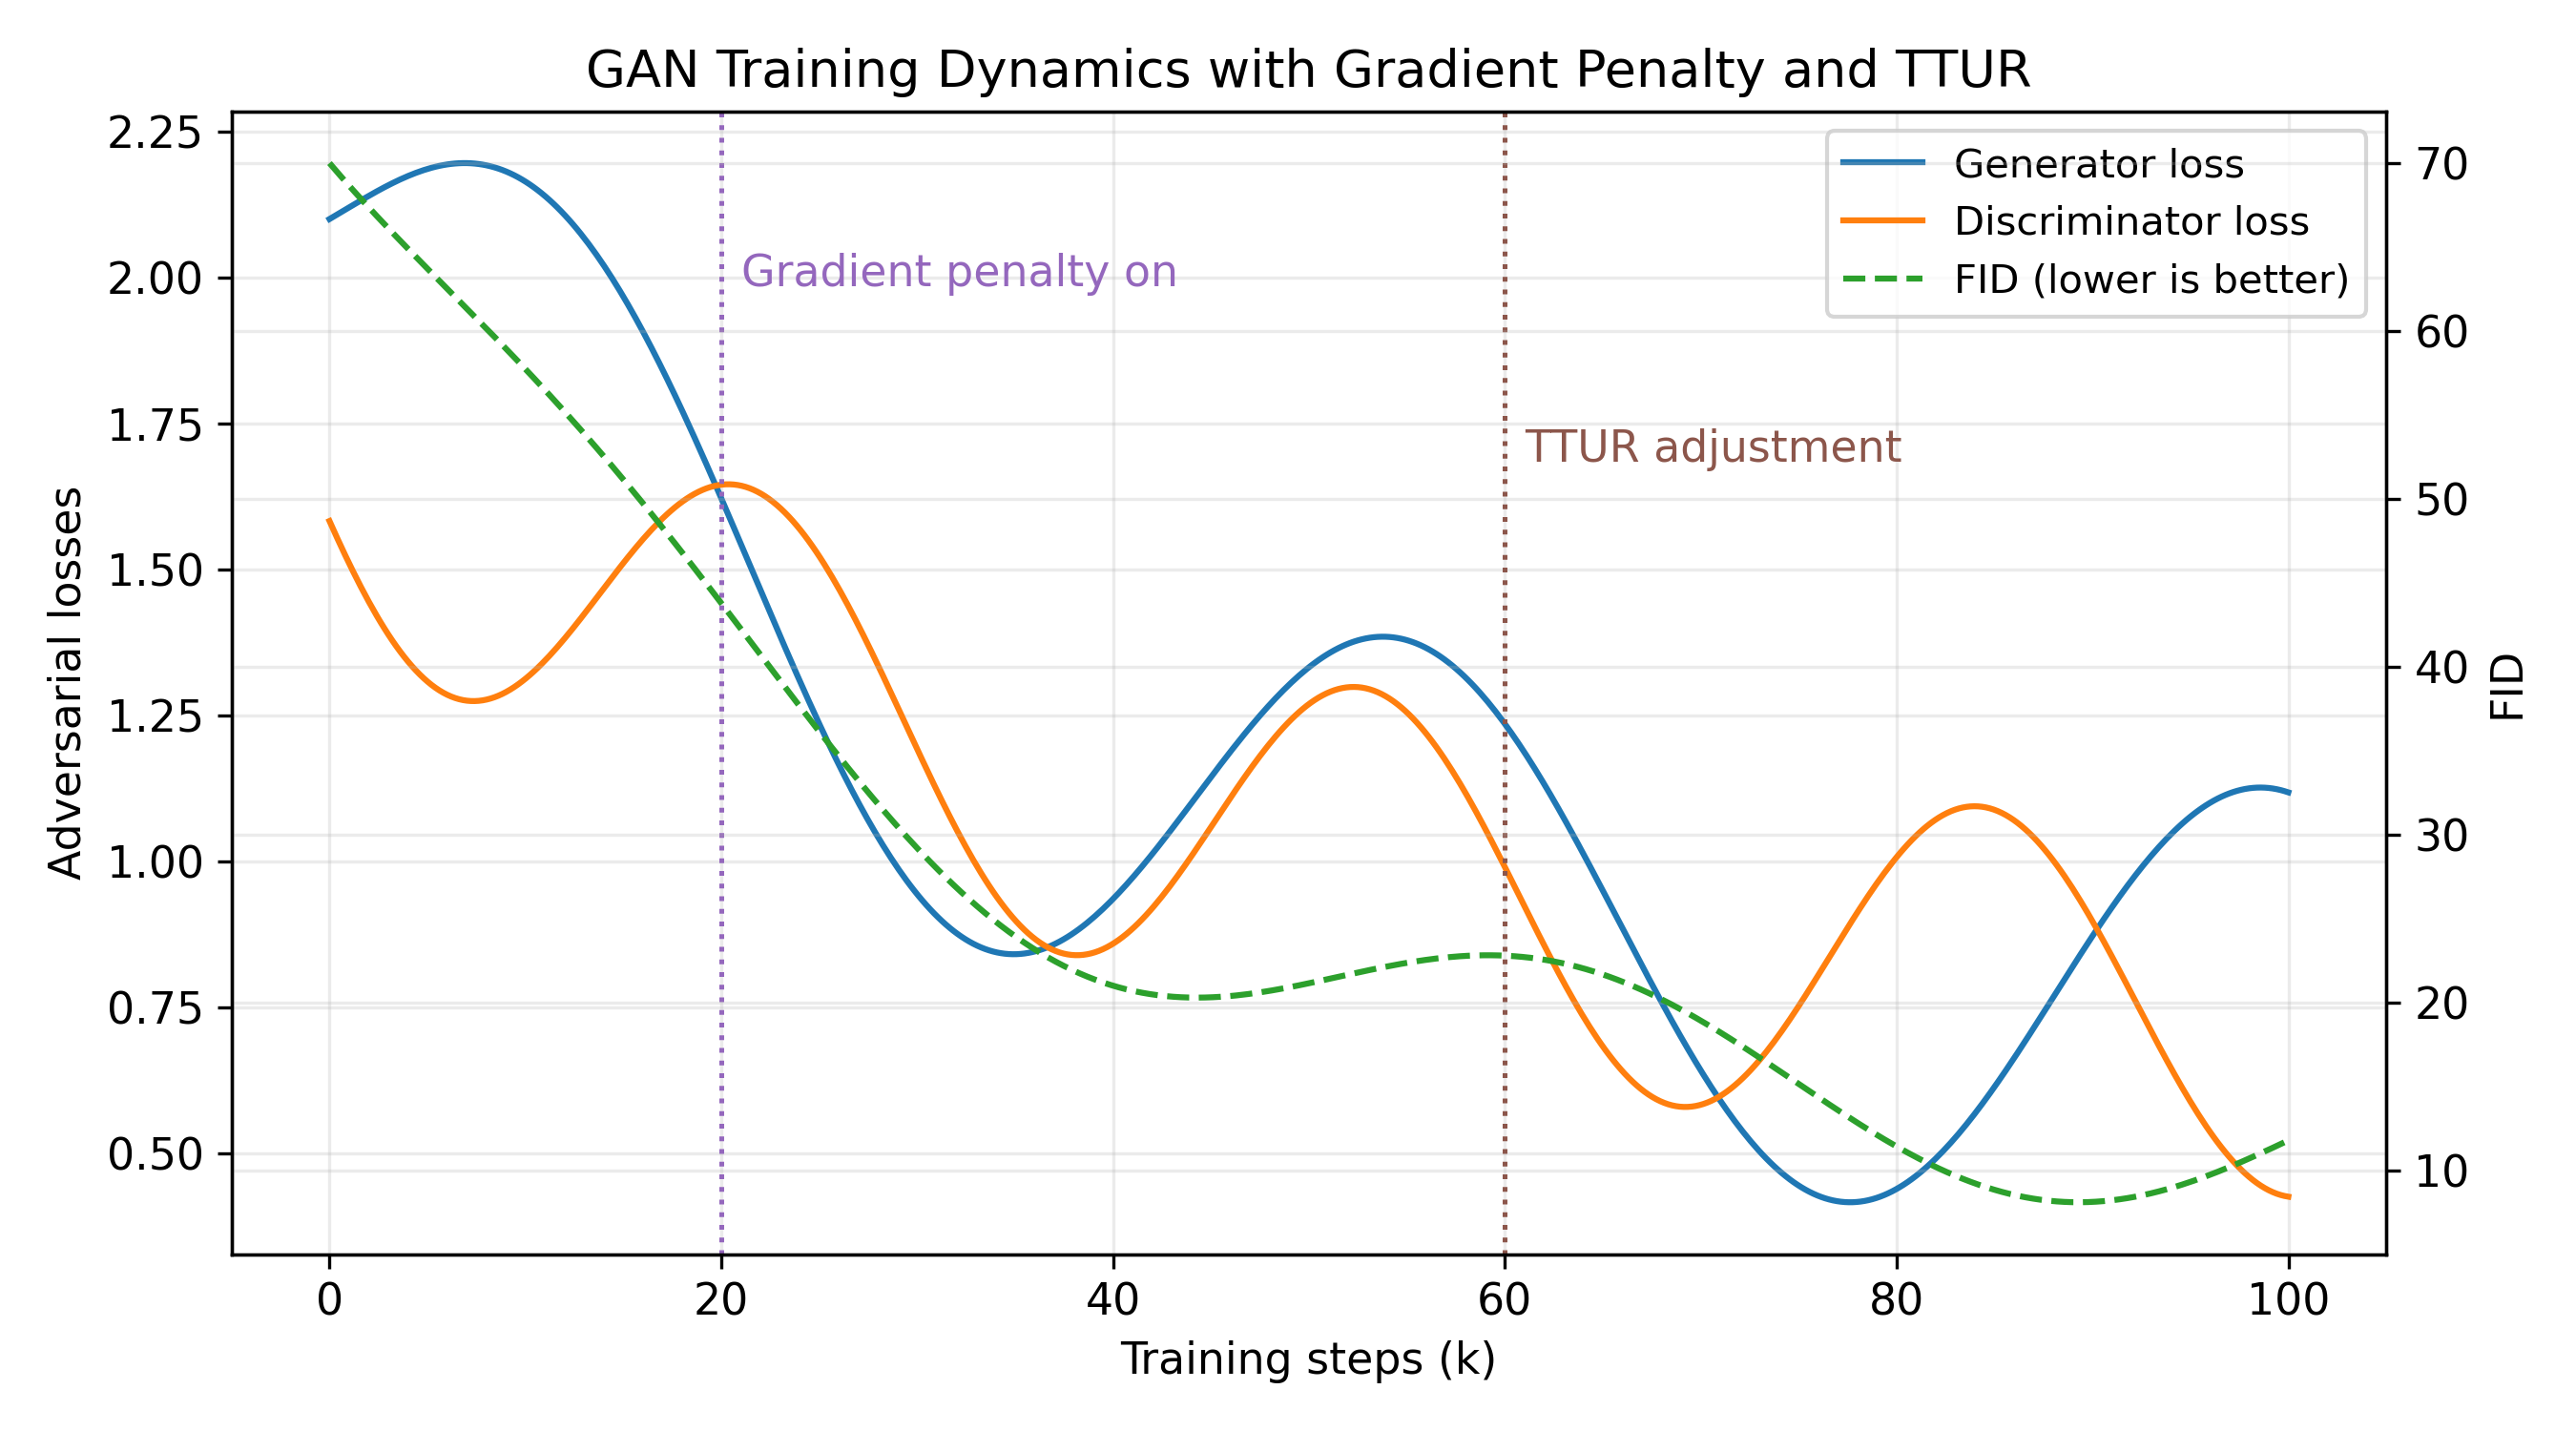
\includegraphics[width=0.85\textwidth]{gan_training_dynamics.png}
  \caption{Generator and discriminator loss trajectories with gradient penalty and TTUR scheduling.}
  \label{fig:gan_training_dynamics}
\end{figure}
\FloatBarrier

\section{Diffusion Models Overview}
Diffusion models generate data by reversing a gradual noising process. The forward process corrupts data $\mathbf{x}_0$ into $\mathbf{x}_T$ using a variance schedule $\{\beta_t\}_{t=1}^{T}$:
\begin{equation}
  q(\mathbf{x}_t \mid \mathbf{x}_{t-1}) = \mathcal{N}\bigl(\sqrt{1 - \beta_t}\,\mathbf{x}_{t-1}, \beta_t \mathbf{I}\bigr).
\end{equation}
Due to Gaussian composition,
\begin{equation}
  q(\mathbf{x}_t \mid \mathbf{x}_0) = \mathcal{N}\bigl(\sqrt{\bar{\alpha}_t}\,\mathbf{x}_0, (1 - \bar{\alpha}_t)\mathbf{I}\bigr), \quad \bar{\alpha}_t = \prod_{s=1}^{t} (1 - \beta_s).
\end{equation}

\subsection{Denoising Diffusion Probabilistic Models (DDPM)}
The model learns $\epsilon_\theta(\mathbf{x}_t, t)$ to predict noise. The simplified training objective is
\begin{equation}
  \mathcal{L}_{\mathrm{simple}} = \mathbb{E}_{t, \mathbf{x}_0, \boldsymbol{\epsilon}} \left[ \|\boldsymbol{\epsilon} - \epsilon_\theta(\sqrt{\bar{\alpha}_t}\mathbf{x}_0 + \sqrt{1 - \bar{\alpha}_t}\,\boldsymbol{\epsilon}, t)\|_2^2 \right].
\end{equation}
Sampling begins from $\mathbf{x}_T \sim \mathcal{N}(\mathbf{0}, \mathbf{I})$ and iteratively denoises:
\begin{equation}
  \mathbf{x}_{t-1} = \frac{1}{\sqrt{1 - \beta_t}} \left( \mathbf{x}_t - \frac{\beta_t}{\sqrt{1 - \bar{\alpha}_t}} \epsilon_\theta(\mathbf{x}_t, t) \right) + \sigma_t \mathbf{z}, \quad \mathbf{z} \sim \mathcal{N}(\mathbf{0}, \mathbf{I}).
\end{equation}
Figure~\ref{fig:diffusion_process} visualizes forward and reverse trajectories.

\subsection{Improvements and Variants}
\begin{itemize}
  \item \textbf{Guided diffusion:} Classifier guidance adjusts sampling drift, $\hat{\epsilon} = \epsilon_\theta - \sigma_t \nabla_{\mathbf{x}_t} \log p_\phi(y \mid \mathbf{x}_t)$, improving class-conditional fidelity.
  \item \textbf{Score-based generative models:} Learn $\nabla_{\mathbf{x}} \log q_t(\mathbf{x})$ with stochastic differential equations (SDEs) and integrate using predictor-corrector samplers.
  \item \textbf{Latent diffusion:} Compress data into latent space via VAE before diffusion (e.g., Stable Diffusion), reducing computational cost while leveraging cross-attention for conditioning.
\end{itemize}

\subsection{Pseudo-code}
\begin{lstlisting}[language=Python, caption={Diffusion training step with cosine noise schedule.}]
def diffusion_training_step(model, scheduler, x0):
    t = torch.randint(0, scheduler.num_steps, (x0.size(0),), device=x0.device)
    noise = torch.randn_like(x0)
    alpha_bar = scheduler.alpha_bar(t).view(-1, 1, 1, 1)
    xt = torch.sqrt(alpha_bar) * x0 + torch.sqrt(1 - alpha_bar) * noise
    noise_pred = model(xt, t)
    loss = (noise - noise_pred).pow(2).mean()
    loss.backward()
    optimizer.step()
    optimizer.zero_grad()
    return loss
\end{lstlisting}

\begin{figure}[H]
  \centering
  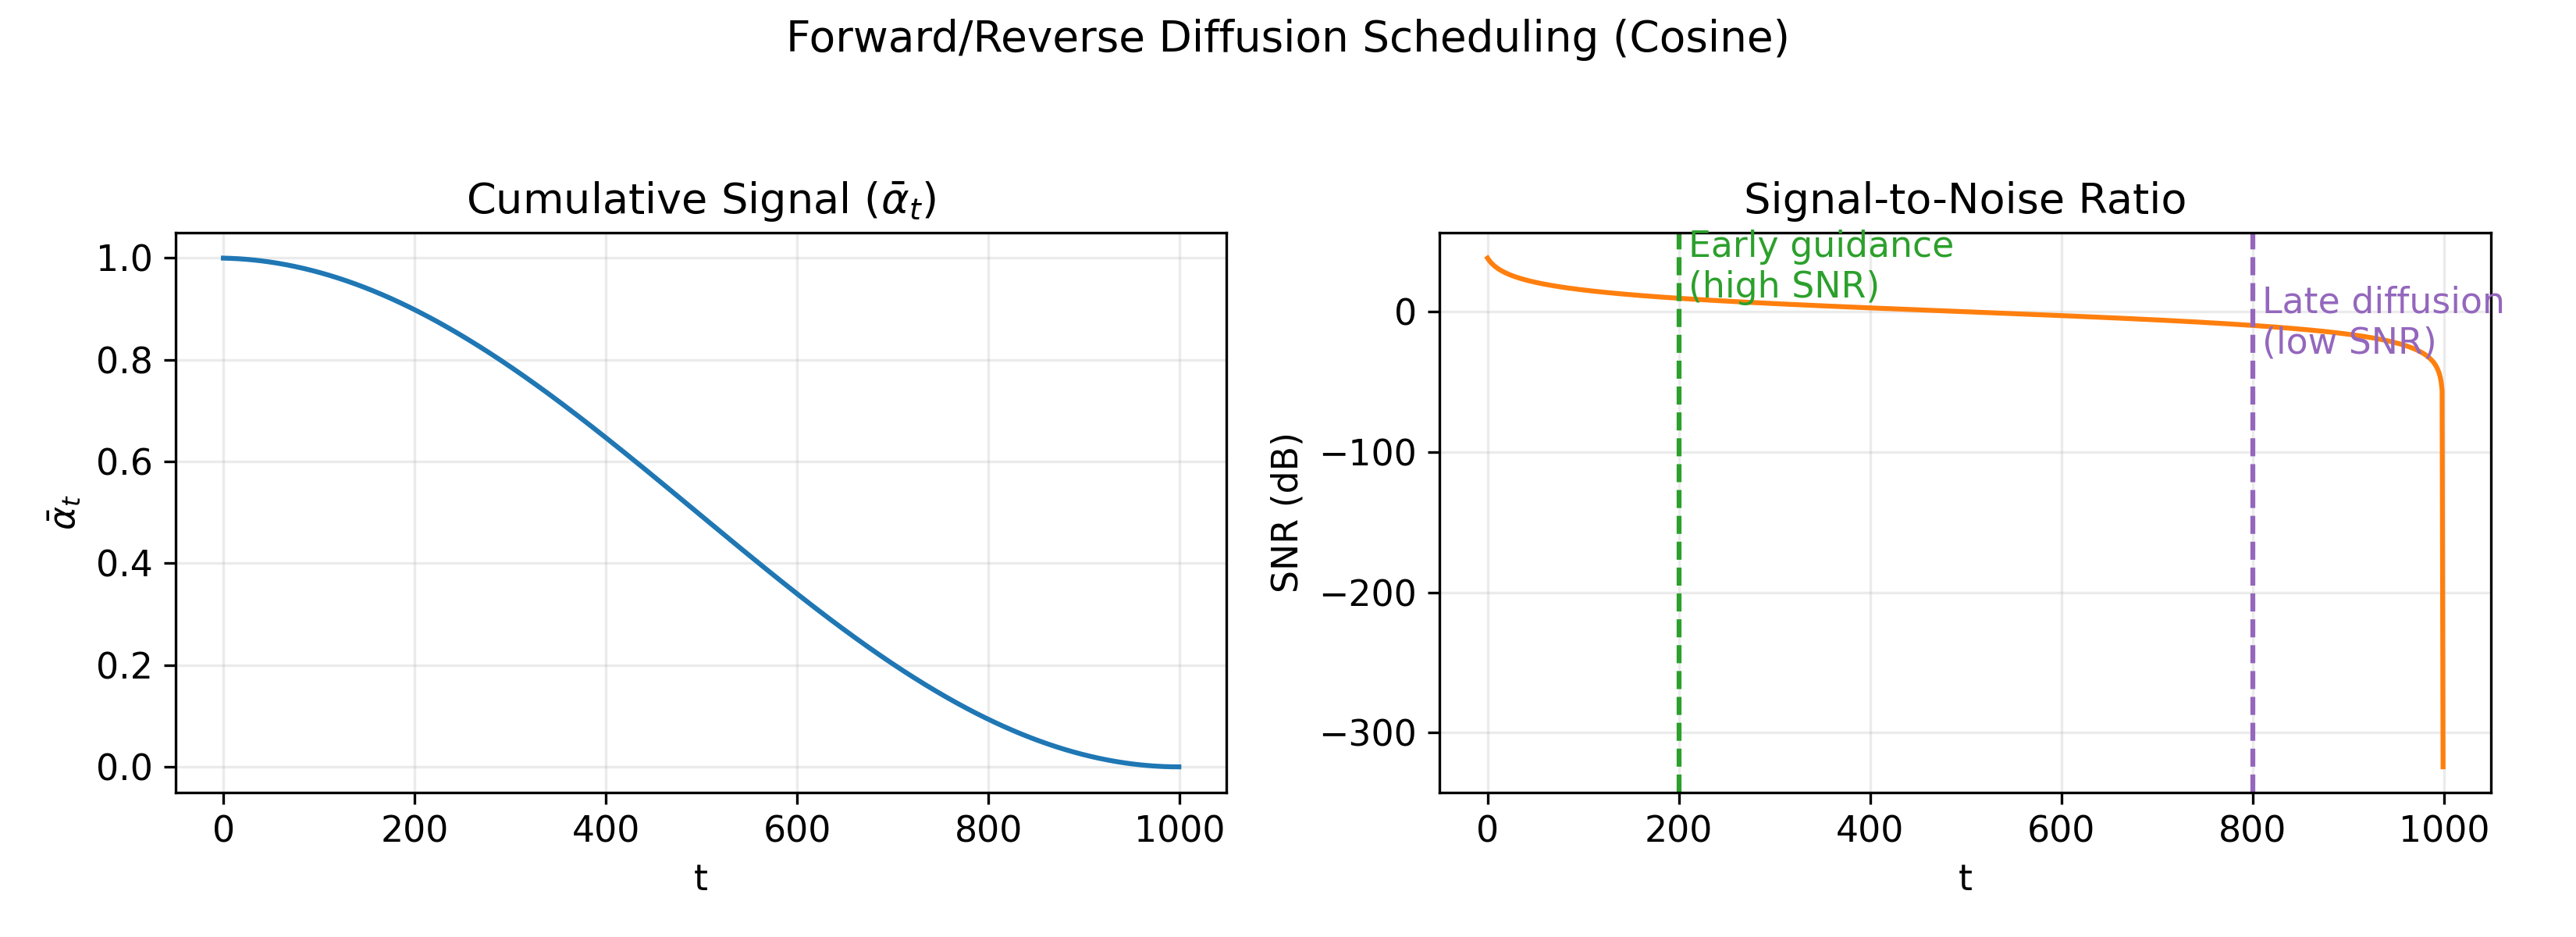
\includegraphics[width=0.85\textwidth]{diffusion_process.png}
  \caption{Forward noising and reverse denoising trajectories in a diffusion model with cosine schedule.}
  \label{fig:diffusion_process}
\end{figure}
\FloatBarrier

\section*{Further Reading}
\begin{itemize}
  \item Diederik P. Kingma and Max Welling. ``Auto-Encoding Variational Bayes.'' ICLR 2014.
  \item Ian Goodfellow et al. ``Generative Adversarial Networks.'' NIPS 2014.
  \item Tero Karras et al. ``Analyzing and Improving the Image Quality of StyleGAN.'' CVPR 2020.
  \item Jonathan Ho et al. ``Denoising Diffusion Probabilistic Models.'' NeurIPS 2020.
  \item Prafulla Dhariwal and Alexander Nichol. ``Diffusion Models Beat GANs on Image Synthesis.'' NeurIPS 2021.
\end{itemize}

\end{document}
